\section{Selfish mining}

In the previous section, we've considered an attack to trick vendors by taking advantage of the system. Now, we will study a method to trick the system itself.

As we mentioned before, a node wins a reward when he successfully mines a block and adds it in the blockchain, the node earns the rewards as long as his block is in the blockchain. \newline

We will present the method of selfish mining, where miners try to increase their rewards allowed for mining (see \cite{majority_not_enough}).

  \subsection{What is it?}

First, let's suppose that all the computational power is divided into two groups: the first group follows the selfish mining strategy and the second group follow the classic mining strategy. \newline

The main idea of selfish mining is to mine secretly blocks in advance so the miners create a longer chain than the others. Then, at the right time, they reveal their chain which will become the new longest chain, so they win the rewards and waste the work of the other miners. \newline

Let's see in details how this strategy works, there are four important cases: \newline

\begin{itemize}
  \item Case 1: The honest miners find a new block on the public chain, the selfish miners will just adopt the new chain.
  \item Case 2: The selfish miners find a new block on the public chain, they will keep this block secret and then, there are two possibilities (Case 3 or 4).
  \item Case 3: The selfish miners have secretly one block in advance but the honest miners find a new block first and broadcast it, in that case, the selfish miners broadcast their secret block immediately. Since two blocks are broadcast almost at the same time, miners will have to choose which block they mine after. All the selfish miners will mine after their block, and the honest miners will mine on the first they receive. Let's note $\gamma$ the proportion of honest miners who mine after the selfish miners' block.
  \item Case 4: The selfish miners have secretly one block in advance and they find a new one, so they keep this new block secret. Then, they will try to keep two blocks or more in advance the longest time possible. If they only have one block left, they publish their secret chain.
\end{itemize}
\medskip

\begin{figure}[ht]
\centering

\subfloat[Case 1]{
  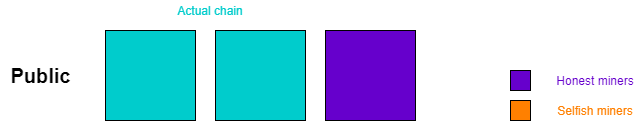
\includegraphics[width=6cm]{Figures/SM_1Honest}
}
\hspace{1cm}
\subfloat[Case 2]{
  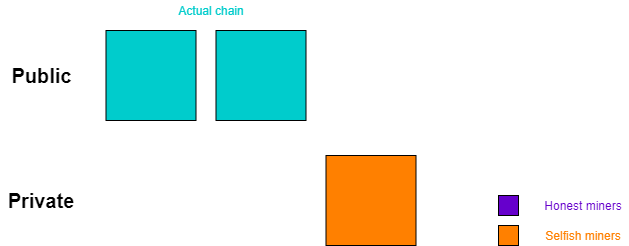
\includegraphics[width=6cm]{Figures/SM_1Selfish}
}
\end{figure}
\medskip

\begin{figure}[ht]
\centering

\subfloat[Case 3]{
  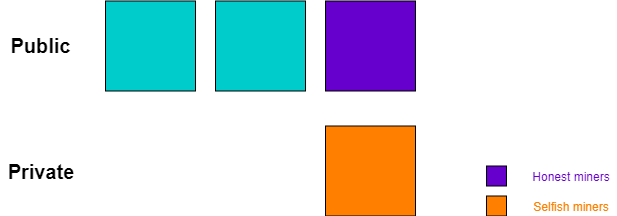
\includegraphics[width=6cm]{Figures/SM_2Honest}
}
\hspace{1cm}
\subfloat[Case 4]{
  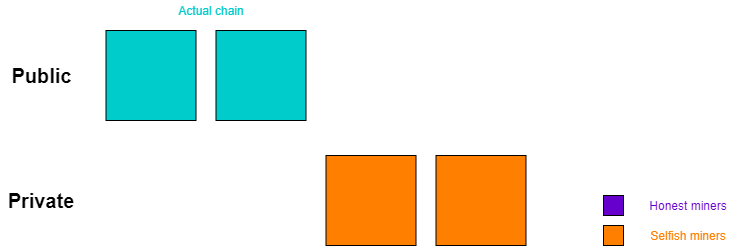
\includegraphics[width=6cm]{Figures/SM_2Selfish}
}
\end{figure}

  \subsection{Is it feasible?}

As we've just seen, this strategy is based on the fact that the selfish miners succeed in mining blocks ahead of the honest miners. To do so, it's obvious that their combined computational power will affect their chance of success, let's note $\alpha$ the computational power of the selfish miners.

As described in \cite{majority_not_enough}, we can represent the selfish mining algorithm with a finite state machine. \newline

\begin{figure}[ht]
\centering
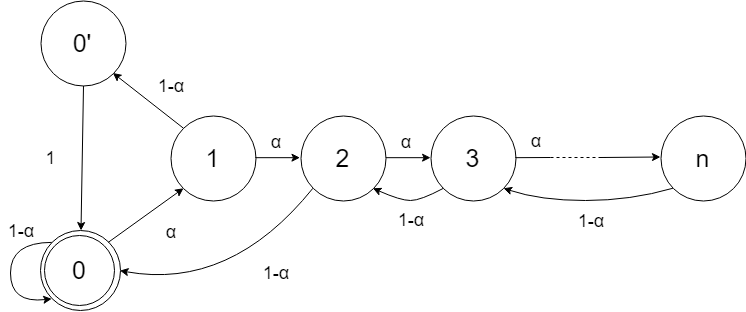
\includegraphics[width=10cm]{Figures/finiteState}
\caption{Selfish mining finite state machine}
\end{figure}
\medskip

In this machine, the initial state is the state 0 and it corresponds to case 1. The state 1 corresponds to case 2, the state 0' to case 3 and the states 2 and more correspond to case 4. \newline

We can compute the probabilities of this state machine, we note $p_i$ the probability of being in state i. From these probabilities, we can compute the rewards the selfish and honest miners will win. \newline

We can find more explanations about the formulas in this appendix \ref{appendixRevenue}. \newline

\begin{table}[ht]
  \centering

  \begin{tabular}{c}
    $r\_honest =  p_0 . (1 - \alpha) . 1 + p_{0'} . \gamma . (1 - \alpha) . 1 + p_{0'} . (1 - \gamma) (1 - \alpha) . 2$ \\
    \\
    $r\_selfish =  p_{0'} . \gamma . (1 - \alpha) . 1 + p_{0'} . \alpha . 2 + p_2 . (1 - \alpha) . 2 + P[i > 2] . (1 - \alpha) . 1$
  \end{tabular}
  \caption{Revenue won by the honest and selfish miners according to $\alpha$ and $\gamma$}
  \label{revenueFormulas}
\end{table}
\medskip

We can implement this finite state machine and try some values of $\alpha$ and $\gamma$.

\begin{figure}[ht]
\centering
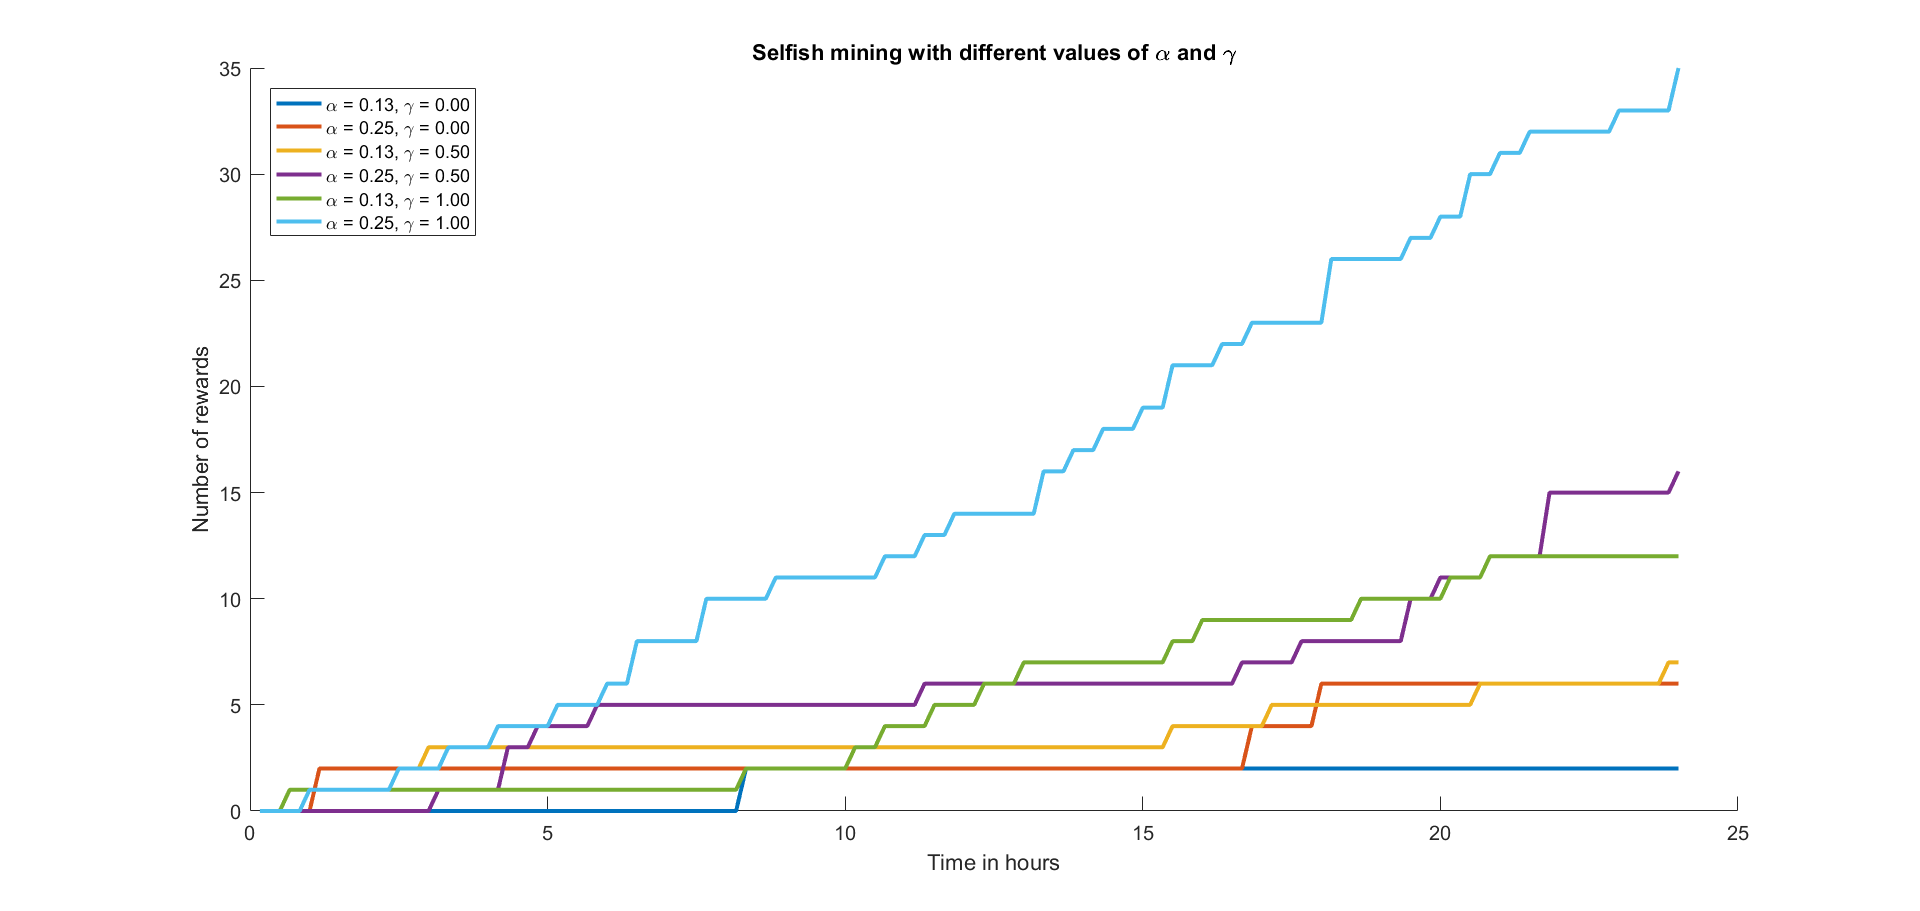
\includegraphics[width=12cm]{Figures/selfishGraph}
\caption{Rewards according to different $\alpha$ and $\gamma$}
\end{figure}
\medskip

We see that $\gamma$ and $\alpha$ are linked because the more $\gamma$ increases the more the pool size $\alpha$ needs to increase to win the same reward. Let's try several values of $\gamma$ with the hash rates of the four largest pools in Bitcoin network (see \cite{hashrate_pools}).

\begin{figure}[ht]
\centering

\subfloat{
  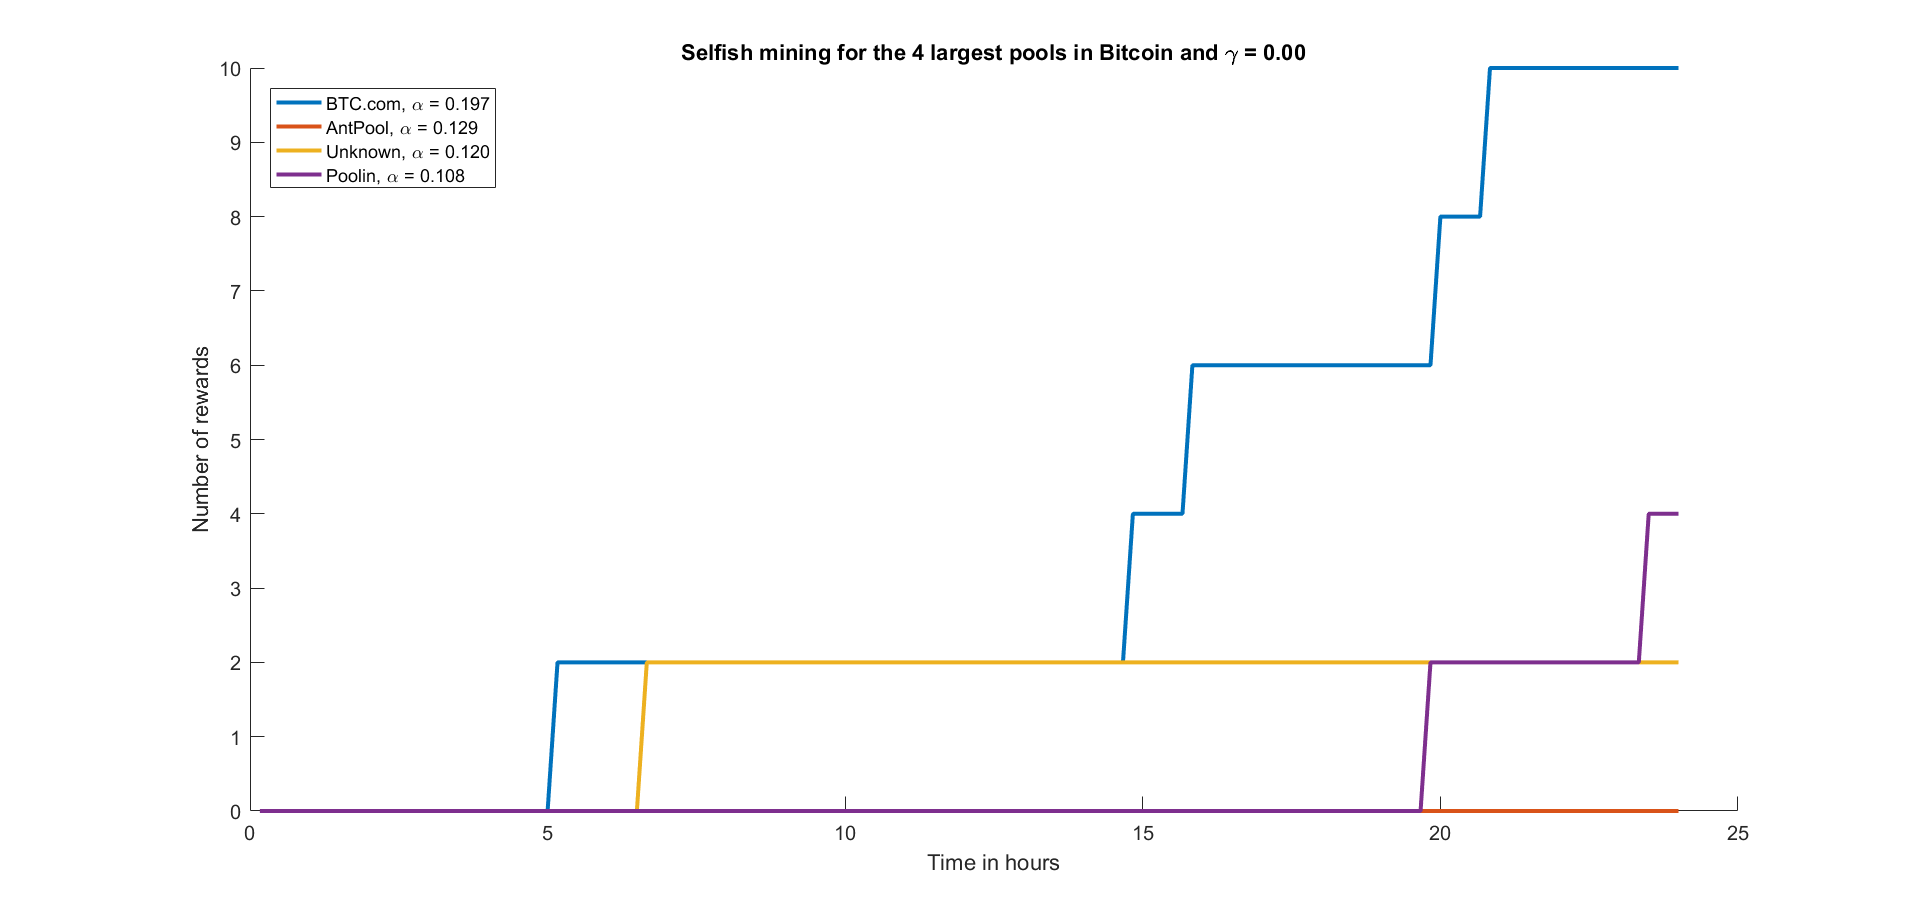
\includegraphics[width=12cm]{Figures/largestPools0}
} \newline

\vspace{1cm}

\subfloat{
  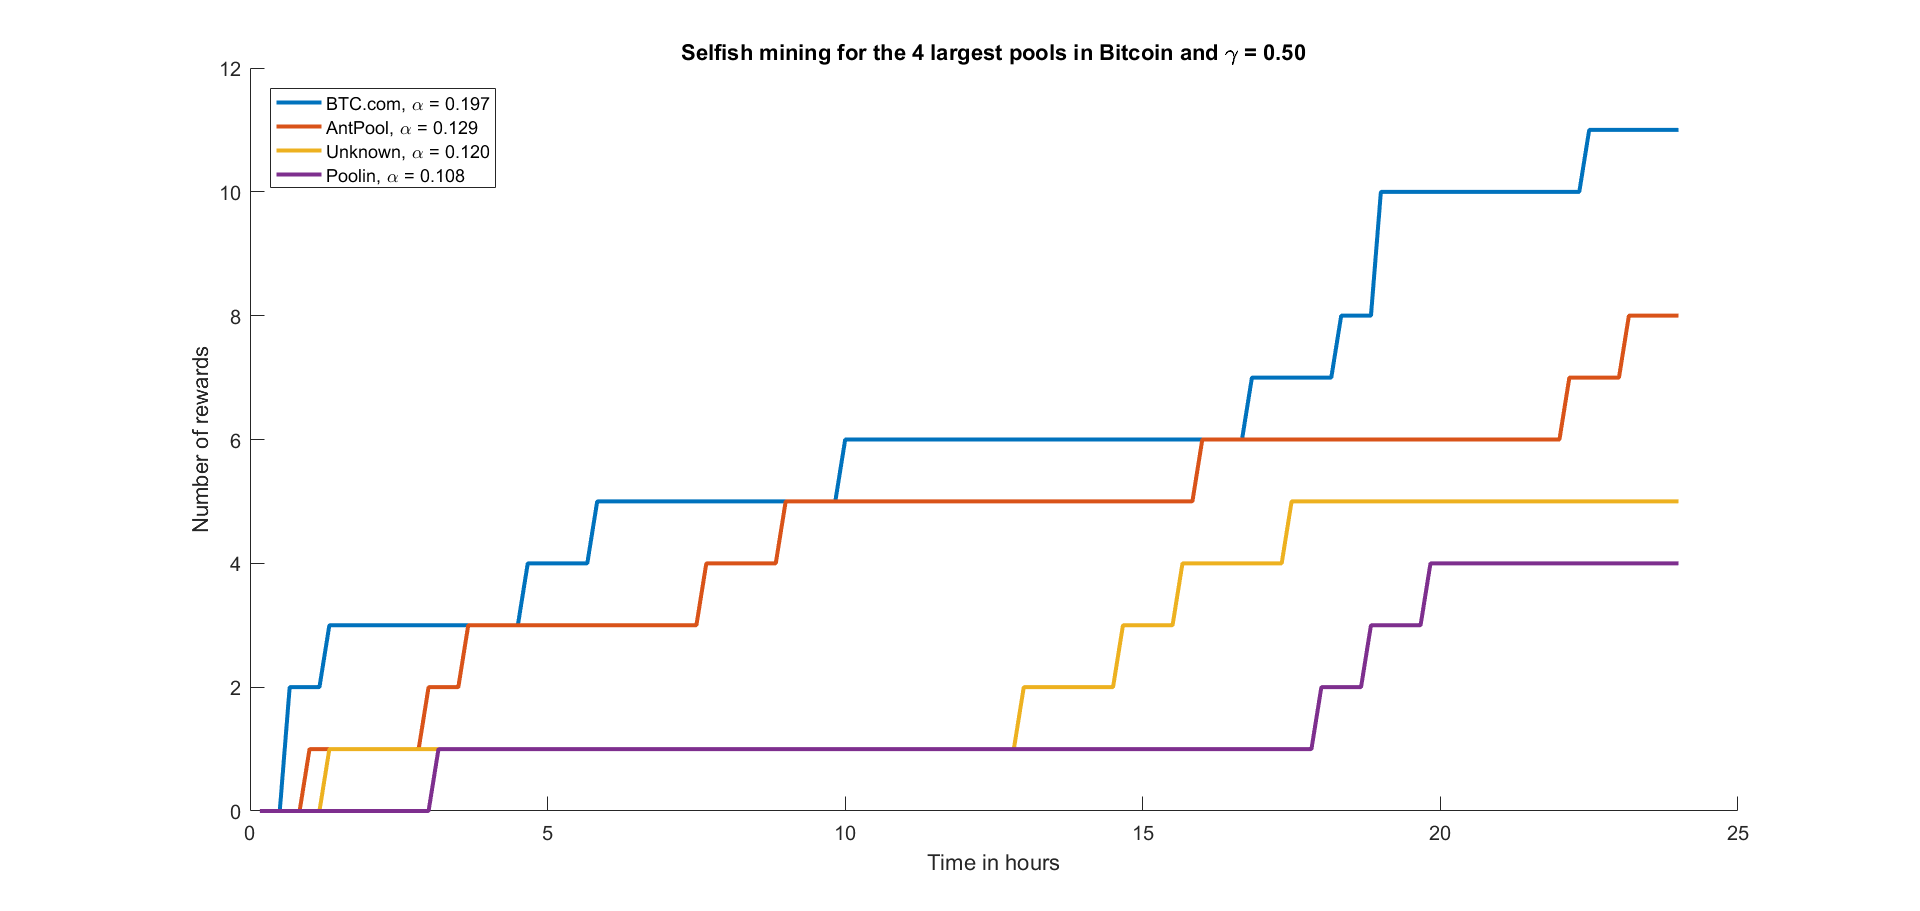
\includegraphics[width=12cm]{Figures/largestPools12}
} \newline
\end{figure}

\begin{figure}[ht]
\centering
\subfloat{
  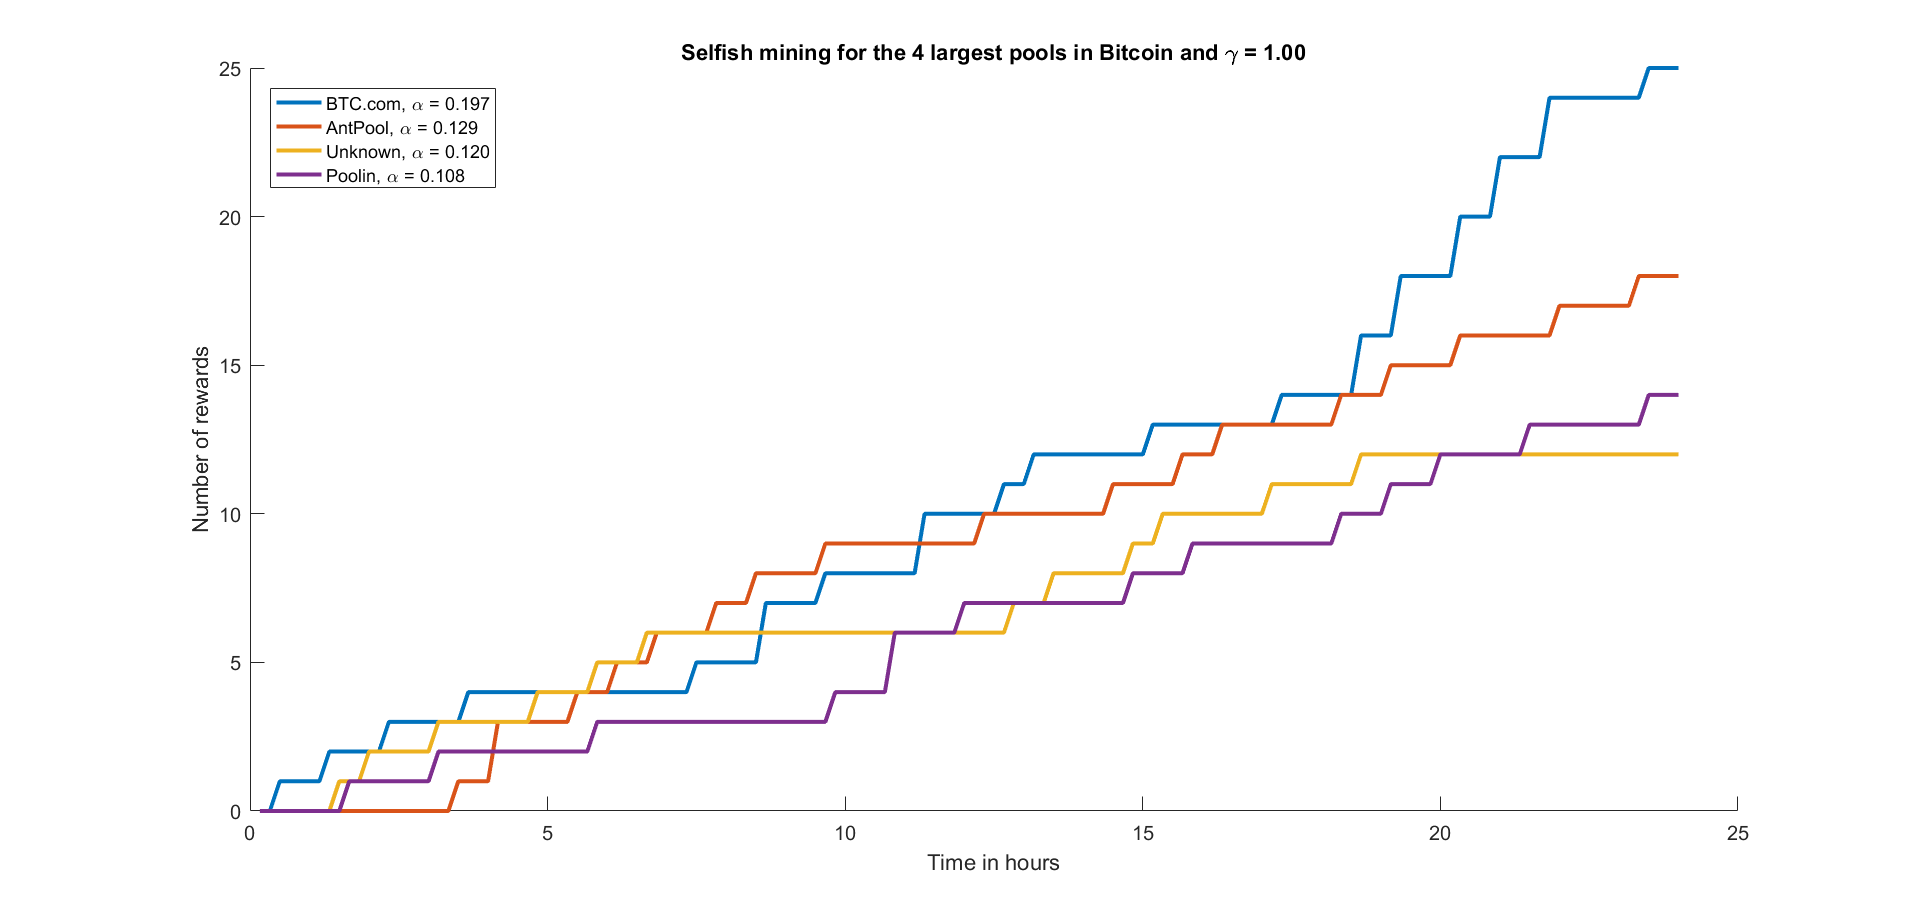
\includegraphics[width=12cm]{Figures/largestPools1}
} \newline
\end{figure}
\medskip

\clearpage
We can see that the pools will be able to win more if they can propagate their blocks fast enough, i.e. if $\gamma$ is high enough.

Now, we need to know if it's worth the effort against the honest mining, to do so we can analyze the link between $\alpha$ and $\gamma$ in the formulas for the revenues (Table \ref{revenueFormulas}) as it was done in \cite{majority_not_enough}. \newline

\begin{figure}[ht]
\centering
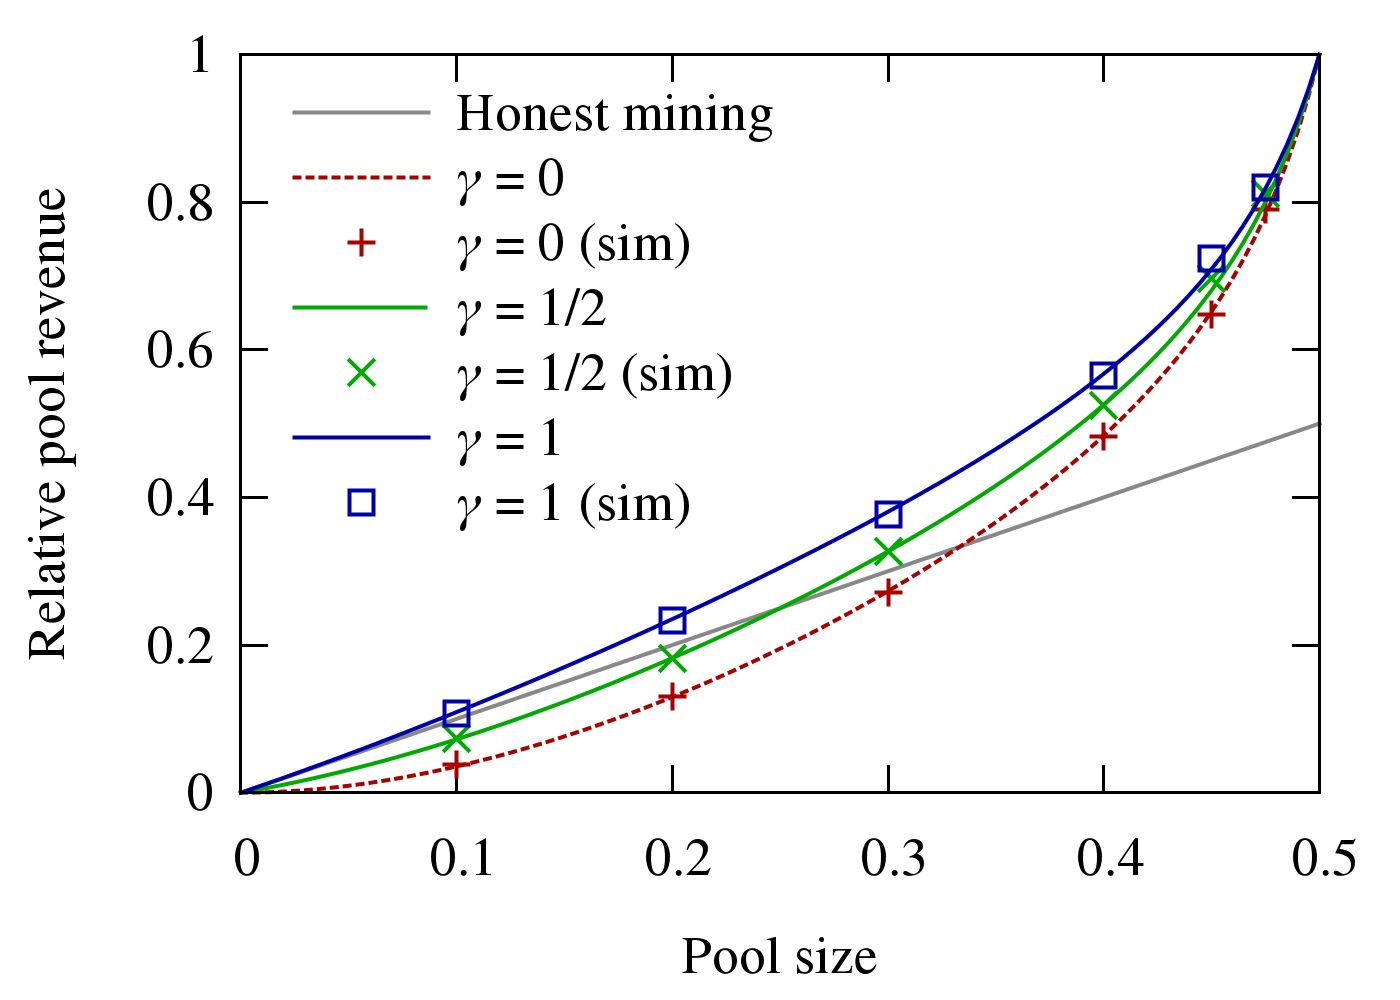
\includegraphics[width=10cm]{Figures/poolRevenue}
\caption{Revenue of the selfish miners for different values of $\alpha$ and $\gamma$}
\end{figure}
\medskip

This figure shows the importance of $\gamma$. With a high $\gamma$, the pool will propagate its blocks to the whole network very quickly so the selfish mining strategy will be efficient.

However, with a low $\gamma$, the honest miners will propagate their blocks quickly. If we take the extreme case of $\gamma = 0$, we'll need a pool with around 35\% of the mining power. For Bitcoin, the largest pool has 19.7\% of hash rate (see \cite{hashrate_pools}) so it seems secured for low $\gamma$.\newline

In Bitcoin, the protocol doesn't ensure that $\gamma$, which represents the propagation rate of the pools' miners, will stay low. This is because when an honest miner has several chains of the same length, he will choose to mine the first block he receives. Then, a pool can perform a Sybil attack, they use virtual miners who won't mine but when they detect that the honest miners have mined a new block, they propagate the pool's block so it will be broadcast faster and increase $\gamma$. \newline

A solution to this problem would be to change the protocol and make the miners to choose randomly between chains of the same length. This would lead to $\gamma = 1/2$ and it would require a pool with 25\% of hash rate, which is hard to achieve.
